\documentclass{standalone}


\usepackage{tikz}
\usetikzlibrary{shapes.geometric, arrows}
\usetikzlibrary{positioning}


\tikzstyle{startstop} = [rectangle, rounded corners, minimum width=2cm, minimum
height=0.5cm,text centered, draw=black]

\tikzstyle{io} = [trapezium, trapezium left angle=70, trapezium right angle=110, minimum
width=2.5cm, minimum height=0.5cm, text centered, text width = 1.5cm, draw=black]

\tikzstyle{process} = [rectangle, minimum width=2cm, minimum height=0.5cm, text centered,
text width = 1cm, draw=black]
\tikzstyle{decision} = [diamond, minimum width=2cm, minimum height=0.5cm, text centered,
draw=black]

\tikzstyle{block1} = [rectangle, rounded corners, minimum width=0.5cm, minimum
height=0.25cm,text centered, draw=black]

\tikzstyle{block2} = [rectangle, rounded corners, minimum width=2.5cm, minimum
height=3.6cm,text centered, draw=black]



\tikzstyle{arrow} = [thick,->,>=stealth]



\begin{document}
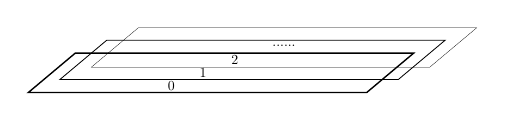
\begin{tikzpicture}[node distance=1cm, thick]
  \node (sheet0) [io, trapezium left angle=40, trapezium right angle=140, minimum
  height=.5cm, minimum width=1.5cm, line width=0.05em, label={[anchor=south
    west, inner sep=1.5pt, scale=.5, xshift=-.9cm]south west:$0$}] {};

  \node (sheet1) [io, above=of sheet0, yshift=-1.35cm, xshift=.4cm, trapezium left angle=40, trapezium right angle=140, minimum
  height=.5cm, minimum width=1.5cm, line width=0.03em, label={[anchor=south
    west, inner sep=1.5pt, scale=.5, xshift=-.9cm]south west:$1$}] {};

  \node (sheet2) [io, above=of sheet1, yshift=-1.35cm, xshift=.4cm, trapezium left angle=40, trapezium right angle=140, minimum
  height=.5cm, minimum width=1.5cm, line width=0.01em, label={[anchor=south
    west, inner sep=1.5pt, scale=.5, xshift=-.9cm]south west:$2$}] {};

  \node (more) [above=of sheet2, yshift=-1.3cm, xshift=0cm, scale=.5] {......};

  

\end{tikzpicture}
\end{document}


%%% Local Variables:
%%% mode: latex
%%% TeX-master: t
%%% End:
